\documentclass{article}
\title{Group Assignment 2}
\author{Odo Chinagorom. Reg  No:2018/249040 }
\usepackage{graphicx}
\begin{document}
\maketitle
\newpage

%\Question 1
\section*{Problem 2.1, page 72}
\begin{center} Solution \end{center}
\[L = 80m\]
\[d = 5mm 5 \times 10^{-3}m\]
\[E = 200GPa = 200 \times 10^{9}\]
\[\sigma_{uth} = 400MPa = 400 \times 10^{6}\]
\[ n = 3.2\]
\begin{itemize}
\item \[\sigma_{uth} = \frac{P}{A}\]
\[P = \sigma_{allow} \times A\]
\begin{center} but $\sigma_{allow} = \frac{\sigma_{uth}}{n} = \frac{400 \times 10^{6}}{3.2} = 1.25 \times 10^{6}Pa$\end{center}
\[P_{ult} = 125 \times 10^{6} \times A\]
\[Area, A=\frac{\pi}{4} \times{5 \times 10^{-3}}^{2} = 1.963 \times 10^{-5}\]
\[P_{ult} = 125\times 10^{6} \times 1.963 \times 10 ^{-5}\]
\[p = 2453.26N\]
\item Elongation  of the wire, $\delta$
\[\delta = \frac{PL}{AE} = \frac{2453.75 \times 80}{200\times10^{9}\times1.963\times10^{-5}}\]
\[=0.05m\]
\end{itemize}


%\Question 2
\section*{Question 2.9}
\begin{center} Solution\end{center}
\[ \delta = 0.08in\]
\[P = 500lb(tensile)\]
\[\sigma_{ult} = 22ksi = 22 \times 10^{3}psi\]
\[E = 10.1 \times 10^{6} psi\]
\begin{center}smallest diameter, d=?\end{center}
\begin{center} Shortest Length, l = ? \end{center}
\begin{center} but $ E = \frac{\delta}{L}$\end{center}
\begin{center} Make L subject of the formular\end{center}

\[L = \frac{\delta}{E} ----------equ(1)\]
\begin{center} $E =\frac{\sigma}{e}. Therefore, e = \frac{\sigma}{E}$\end{center}
\[E = \frac{22 \times10^{3}}{10.1\times10^{6}} = 2.18\times 10^{-3}\]
\begin{center}Substituting the value of E into the equation 1\end{center}
\[L = \frac{0.08}{2.18\times10^{-3}}=36.7in\]
Smallest Diameter $d_{1}$ ,
\[A = \frac{\pi}{4}d^{2}\]
\begin{center} Therefore, $d = 2 \times \sqrt{\frac{A}{\pi}}$\end{center}
but A is unknown. So to find A, 
\[\delta = \frac{PL}{AE} = \frac{500 \times 36.7}{A \times 10.1\times10^{6}} = 0.08\]
Therefore, A will be
\[A = \frac{500\times36.7}{0.08\times10.1\times10^{6}} = 0.0227\]
\[d = \sqrt{\frac{0.0227}{\pi}} = 0.17in\]

%\Question 3
\section*{Question 2.15}
\begin{center} Solution\end{center}
Given:
\[ L_{BA} = 4ft = 4 \times 12 = 48in\]
\[ L_{AC} = 3ft = 3 \times 12 = 36in\]
\[ L_{BC} = 7ft = 7 \times 12 = 84in\]
\[ A_{BA} =  1.75in_{2}\]
\[d_{BC} = \frac{5}{8}in\]
\[ E_{s} = 29 \times 10^{6}psi, \space E_{D} = 10.4 \times 10^{6}psi\]
\[p = 15Kip = 15\times 10^{3}lb\]
Deflection at point c, $\delta_{c} = \delta_{BC} + \delta_{BA}$
\[\delta_{BC} = \frac{L_{BC}P}{A_{BC}E_{s}} \]
\[A_{BC} = \frac{\pi}{4} \times {(\frac{5}{8})^{2}} = 0.307in^{2}\]
\[\delta_{BC} = \frac{15 \times 10^{3}\times 84}{0.307 \times 29 \times 10^{6}} = 0.1415in\]
\[\delta_{BA} = \frac{PL_{BA}}{A_{BA}E_{D}} = \frac{15 \times 10^{3}\times48}{1.75\times10.4\times10^{6} }= 0.03956\]
\[\delta = 0.1415 + 0.03956 = 0.18106in\]

%\Question 4
\section*{Question 2.19}
\begin{center} Solution\end{center}
Given: 
\[E = 70GPa = 70 \times 10^{9}Pa\]
\[P = 4KN = 4 \times 10^{3}N\]
\[d_{DB} = 20mm. \space \space d_{BC} = 6mm. \space \space d_{AB} = 0.4mm. \space \space d_{B2} = 0.5m. \space \space\]
For deflection at A to be 0,\[\delta_{AB} = \delta_{BC}\]
\[A_{AB} = \frac{\pi}{4}d^{2} = \frac{\pi}{4}{20\times 10^{-3}}^2 = 3.24  \times 10^{-4}m^{2}\]
\[A_{BC} = \frac{\pi}{4}d^{2} = \frac{\pi}{4}{60\times 10^{-3}}^2 = 2.827  \times 10^{-3}m^{2}\]
\[\delta_{AB} = \frac{PL_{AB}}{A_{AB}E} = \frac{4\times 10^{3} \times 0.4}{3.14 \times 10^{-4} \times 70 \times 10^{9}}= 7.279\times10^{-6} \]
\[\delta_{BC} = \frac{(Q-P)L_{BC}}{A_{BC}E} = \frac{(Q-P) \times 0.5}{2.827 \times 10^{-3} \times 70 \times 10^{9}}\]
\[=\frac{(Q-4000)0.5}{2.125 \times 10^{-3}\times 70 \times 10^{9}} = \frac{0.5Q - 2000}{1.9789 \times10^{4}}\]
Since, \[\delta_{AB} = \delta_{BC}\]
then\[7.279\times10^{-6} = \frac{0.5Q - 2000}{19789 \times 10^{-4}}\]
\[0.5Q - 2000 = 7.279\times19789\times10^{4} = 1440.44\]
\[0.5Q= 1440.44+2000\]
\[0.5Q = 3440.44\]
\[q = \frac{3440.44}{0.5} = 6880.88N\]

Corresponding deflection at A
\[\delta_{BC} = \delta_{AC}= 7.279\times10^{-6}\]




%\Question 5
\section*{Question 2.26}
\begin{center} Solution\end{center}
Given:
\begin{center}Length of string,$ L_{s} = 12.5 in$\end{center}
\begin{center}diameter of string,$d_{s} = \frac{3}{32}in$\end{center}
\begin{center}$E_{S} = 29 \times 10^{6}$\end{center}
\begin{center}$P = 50lb$\end{center}
Drawing a free body diagram of the syste, we have \newline
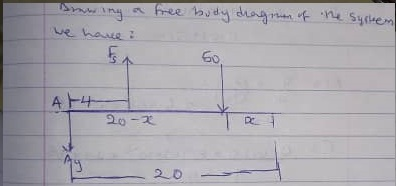
\includegraphics{IMG-20220126-WA0004}\newline
Taking moment about point A, we have
\[M_{A} = 4f_{s} - 50 (20 -x) = 0\]
but $f_{s} = ?$, However
\begin{center}$\delta_{s} = \frac{f_{s}L_{s}}{A_{s}E}$.  This implies that $f_{s} = \frac{\delta_{s}A_{s}E}{L_{s}}$\end{center}
\[\delta_{s} = 4 \theta\]
where 4 is th edistance fro the string to the point A
\newline
$\theta$ is the angle covered by the beam
\[\theta = \frac{\frac{1}{16}}{20} = 3.125 \times 10^{-3}rads\]
\[\delta_{s} = 4\times 3.235 \times 10^{-2} = 0.065in\]
\[A_{s} = \frac{\pi}{4} \times (\frac{3}{32})^{2} = 6.903 \times 10^{-3}in^{2}\]
\[F = \frac{0.0125 \times 6.903 \times 10^{-3} \times 29 \times 10^{6}}{12.5} = 200187lbs\]
Hence,
\[4f_{s} - 50(20-x) = 0\]
\[(4\times200.187) - 1000 + 50x = 0\]
\[800.748 - 1000 + 50x = 0\]
\[50x = 199252\]
\[ x = \frac{199.252}{50}\]
\[x = 3.985in\]


%\Question 6
\section*{Question 2.35}
\begin{center} Solution\end{center}
\begin{center}$ P = P_{c} + P_{s}$\end{center}
deformation of a steel bar and that of a concrete are equal, hence
\[\delta_{c} = \delta_{s}\]
\[\frac{P_{c}L_{c}}{A_{c}E_{c}} = \frac{P_{s}L_{s}}{A_{s}E_{s}}\]
making $P_{c}$ the subject of the formular, we have
\[P_{c} = \frac{P_{s}A_{c}E_{c}}{A_{s}E_{s}}\]
\[A_{s} = 4\times\frac{\pi}{4} \times(\frac{3}{4})^{2} = 1.767in^{2}\]
\[A_{s} = 8_{2} - A_{s}= 64 - 1.767 = 62.233in^{2}\]
Since $P_{c} = \frac{P_{s}A_{c}E_{c}}{A_{s}E_{s}}$
\[P = P_{c} + P_{s}\]
\begin{center} becomes\end{center}
\[P = \frac{P_{s}A_{c}E_{c}}{A_{s}E_{s}} + P_{s}\]
This then becomes
\[P = P_{s}\frac{A_{c}E_{c}}{A_{s}E_{s}} + 1\]
\[P = 150Kips = 180 \times 10^{3}lbs\]
\[150\times10^{3} = P_{s}(\frac{62.233\times3.6\times10^{6}}{1.767\times29\times10^{6}} + 1)\]
\[150 \times 10^{3} = P_{s}(4.372 + 1)\]
\[P_{s} = \frac{150\times10^{3}}{5.372}\]
\[P_{s} = 27922.56lbs\]
Therefore $P_{c} = 50000 - 27922.56 = 122077.44$
Normal Stress:
\[\sigma_{c} = \frac{P_{c}}{A_{c}} = \frac{122077.434}{62.233} = 1961.619psi\]
\[\sigma_{s} = \frac{P_{s}}{A_{s}} = \frac{27922.56}{1767} = 15802.24psi\]




%\Question 7
\section*{Question 2.41}
\begin{center} Solution\end{center}
Considering the reaction at E redundant and realsing the bar from that support and considering the reaction, $R_{E}$ is an unknown lend,

From The above, the total deformation of the bar is
\[\delta =\delta_{AD} + \delta{E} = 0\]
Where $\delta_{AD}$ is as a result of the forces 60KN and 40KN
and $\delta_{E}$ is as a result of the reaction at E
\[\delta_{AD} = \frac{P_{1}L_{1}}{A_{B}E_{B}} + \frac{P_{2}L_{2}}{A_{B}E_{B}} + \frac{P_{3}L_{3}}{A_{S}E_{S}} + \frac{P_{4}L_{4}}{A_{S}E_{S}} \]
Note to get the effect of the forces acting on the rods, the bar was into 4 as shown below
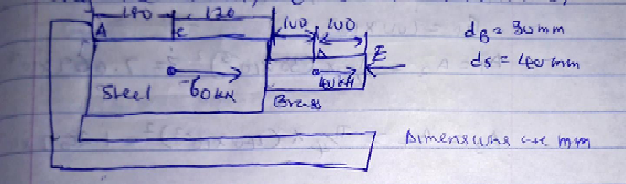
\includegraphics{7}
\[P_{1} = 0, P_{2}=P_{3}=40KN= 40\times10^{3}, p_{4}=100\times10^{3}\]
\[A_{1} = A_{2} = \frac{\pi}{4}\times(30\times10^{-3})^{2}=7.069\times10^{-4}\]
\[A_{3} = A_{4} = \frac{\pi}{4}\times(40\times10^{-3})^{2}=1.257\times10^{-4}\]
\[l_{1} = l_{2} = 100mm = 0.1\]
\[l_{3} = 120mm = 0.12\]
\[l_{4} = 180mm = 0.18\]
\[E_{s} = 200\times 10^{9}, E_{b} = 205\times10^{-3}\]
\[\delta_{AD} = 0 + \frac{40\times0.1\times10^{3}}{7.069\times10^{-3}\times105\times10^{9}}+\frac{40\times10^{3}\times0.12}{1.259\times10^{-3}200\times10^{4}} + \frac{100\times10^{3}\times0.18}{1.257\times10^{-3}\times200\times10^{4}}\]
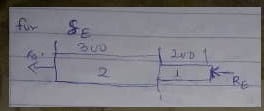
\includegraphics{IMG-20220127-WA0007}
\[=(5.384\times10^{-5}) + (1.909\times10^{-5}) + (7.16\times10^{-5}) = 14.458\times10^{-5}m\]
\[\delta_{E} = \frac{R_{E}\times 0.2}{7.069\times10^{-3}\times105\times10^{9}}+\frac{R_{E}\times0.3}{1.259\times10^{-3}200\times10^{4}}\]
\[=(6.695\times10^{-9}R_{E}) + (1.193\times10^{-3}R_{E}) = 3.886\times10^{-9}R_{E}\]
\begin{center} Equating $\delta_{E}$ and $\delta_{AD}$\end{center}
\[\delta_{E}= \delta_{AD}\]
\[ 14.458\times10^{-5}=3.886\times10^{-9}R_{E}\]
\[R_{E} = \frac{14.458\times10^{-5}}{3.886\times10^{-9}} = 37186.21 = 37.19KN\]
For reaction at A, $R_{A}$ we have
\[R_{E}+R_{A} = (40\times10^{3})+(60\times10^{3})\]
\[R_{A} = (100\times10^{3})=37186.21\]
\[=62813.786N\]
Deflection at point C
\[\delta_{C} = \delta_{AB} + \delta_{BC}\]
\[\delta_{C} = \frac{R_{A}L_{4}}{A_{B}E_{B}} + \frac{P_{A}L_{3}}{A_{S}E_{S}}\]
\begin{center} Where $P = R_{A} - 60\times10^{-3}$\end{center}
\[\frac{62813.786 \times 0.18}{1.257\times 10^{-3}\times 200\times 10^{9}}+\frac{(62813.786-60000)\times 0.12}{1.259\times10^{-3}200\times10^{4}}\]
\[(4.497\times10^{-5})+(1.34\times10^{-6})=4.63\times10^{-5}m\]



%\Question 8
\section*{Question 2.58}
\begin{center} Solution\end{center}
Given \[\sigma = -11ksi = -11\times 10^{3}\]
\[T_{1} = 75^{o}F\]
\[Z_{b} = 14in, L_{AC} = 18in\]
\[A_{B} = 2.4in^{2}\]
\[E_{B} = 15\times10^{6}psi\]
\[\alpha_{B}=15\times10^{-6}F^{-1}\]
\[A_{AC} = 2.8in^{2}\]
\[E_{AC} = 10.6\times10^{6}psi\]
\[\alpha_{AC}=12.9\times10^{-6}F^{-1}\]
\begin{center}Pressure,$P = -\sigma_{AL}A_{AL}=- (11\times10^{3})(2.8) = -30800N$\end{center}
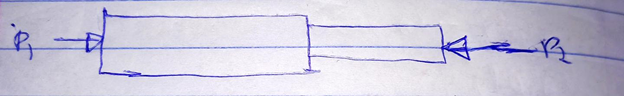
\includegraphics{10}
\[p_{1} = P_{2} = P\]
deformation as a result of force, P
\[F_{P} = \frac{P_{1}L_{B}}{A_{B}E_{B}} + \frac{P_{2}L_{AL}}{A_{AL}E_{AL}}\]
\[=\frac{-30800\times14}{2.4\times15\times10^{6}} + \frac{-30800\times18}{2.8\times10.6\times10^{6}}\]
\[=-0.012 - 0.0187 = -0.0307in\]
This shows that the force $F_{1}$ and $F_{2}$ are compressive forces and the deformation is compression.
\newline
Hence, $\delta_{P} = 0.0307$
Deformation due to the thermal stress,
\[f_{T} = \delta_{P}+\delta = 0.0307 + 0.02 = 0.0507\]
\begin{center}But $F_{T} = \alpha_{B}\triangle T L_{B} +  \alpha_{AL}\triangle T L_{AL}$\end{center}
\[= \triangle T( \alpha_{B} L_{B} +  \alpha_{AL} L_{AL})\]
\[\triangle T(1.2\times 10^{-6}\times14 + 12.9\times10^{-6}\times18)\]
\[=\triangle T(4.002\times10^{-4})\]
\begin{center} Equating it$ \delta_{T} = 0.0507$, we have\end{center}
\[\triangle T(4.002\times20^{-4}) = 0.0507\]
\[\triangle T = \frac{0.0507}{4.002\times10^{-4}} = 126.69\]
$T_{2}$, new temperature for stress of $-11ksi$ to be experienced by aluminium = $\triangle T +T_{1}$
\[=126.69 + 75\]
\[T_{2} = 201.68^{o}F\]
\newline
\newline
Corresponding exact length of aluminum bar
\[F_{A} = L_{AL}\alpha_{AL}(\triangle T) - \frac{PL_{AL}}{E_{AL}A_{AL}}\]
\[=(18)(2.9\times10^{-6})(26.6) = \frac{30800\times 18}{10.6\times10^{6}\times2.8} = 10.712\times10^{-3}\]
\[L_{exact} = 18 + 10.712\times 10^{-3} = 18.0107in\]



%\Question 9
\section*{Question 2.65}
\begin{center} Solution\end{center}
\[length, L = 2.5m\]
\[Outside\space diameter, d_{0} = 300mm = 0.3m\]
\[thickness, t =15mm = 0.015m\]
\[E = 200GPa = 200\times10^{9}Pa\]
\[v=0.30\]
\[P = 700KN = 700\times10^{3}N\]
\begin{itemize}
\item Change in length of the pipe,$\delta$
\[\delta  = \frac{-PL}{AE}\]
\[Area, A = \frac{\pi}{4}\times({{d_{0}}^{2}} - {{d_{1}}^{2}})\]
\[d_{1} = d_{0} - 2t = 0.3-2(0.15)=0.27\]
\[A = \frac{\pi}{4}(0.3^{2} - 0.27^{2}) = 0.0134m^{2}\]
\[\delta = \frac{(700\times10^{3})(2.5)}{(0.0134)(200\times10^{9})} = -6.53\times10^{-4}\]
\item Change in the outer diameter $\triangle d_{0}$
\[\triangle d_{0} = E_{lateral} \times d_{0}\]
but 
\[E_{lateral} = -\nu E_{axial}\]
\[E_{axial} = \frac{\delta}{L} = \frac{-6.53\times 10^{-4}}{2.5}=-2.612\times10^{-4}\]
\[E_{lateral} = -(0.30)(-2.612\times10^{-4}) = 7.836\times10^{-6}\]
\[\triangle d_{0} = 7.836\times10^{-5}\times0.3=2.3508\times10^{-5}m\]
\item Change in thickness, $\triangle t$
\[\triangle = E_{lateral} \times t_{0}= 7.836\times10^{-5}\times0.015=11.1754\times10^{-6}m\]

\end{itemize}

%\Question 10
\section*{Question 2.81}
\begin{center}\underline{solution}\end{center}
\[G = 12MPa = 12\times10^{6}\]
\[L - 100mm = 0.1m\]
\[P = 45KN = 45\times10^{3}N\]
\[a = ?, \space b=?\]
\[\tau = 1.4MPa = 1.4\times10^{6}\]
\[\delta = 5mm = 5\times10^{-3}m\]
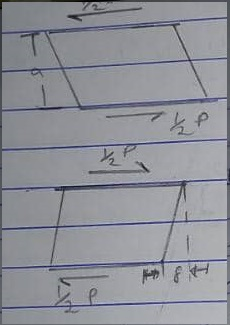
\includegraphics{IMG-20220128-WA0012}
\[F = \frac{1}{2}P = \frac{45\times10^{3}}{2} = 22.5\times10^{3}N\]
Finding b, bc = A but A= ? However\[\tau = \frac{F}{A} \Rightarrow A= \frac{F}{\tau} = \frac{22.5\times10^{3}}{1.4\times10^{6}} = 0.0161m^{2}\]
\[bc=A \Rightarrow b= \frac{A}{C}=\frac{0.0161}{0.1} = 0.1607m\]
Finding a, \[r = \frac{\delta}{a} \Rightarrow a = \frac{\delta}{r}\]
But r is an unknown, However,\[r = \frac{\tau}{G} = \frac{1.4\times10^{6}}{12\times10^{6}}=0.1167\]
subsitituting into $a=\frac{\delta}{r}$
\[a = \frac{5\times10^{-3}}{0.1167} = 0.0428m\]

\end{document}